\section{Übertragung von digitalen Signalen S. 93}
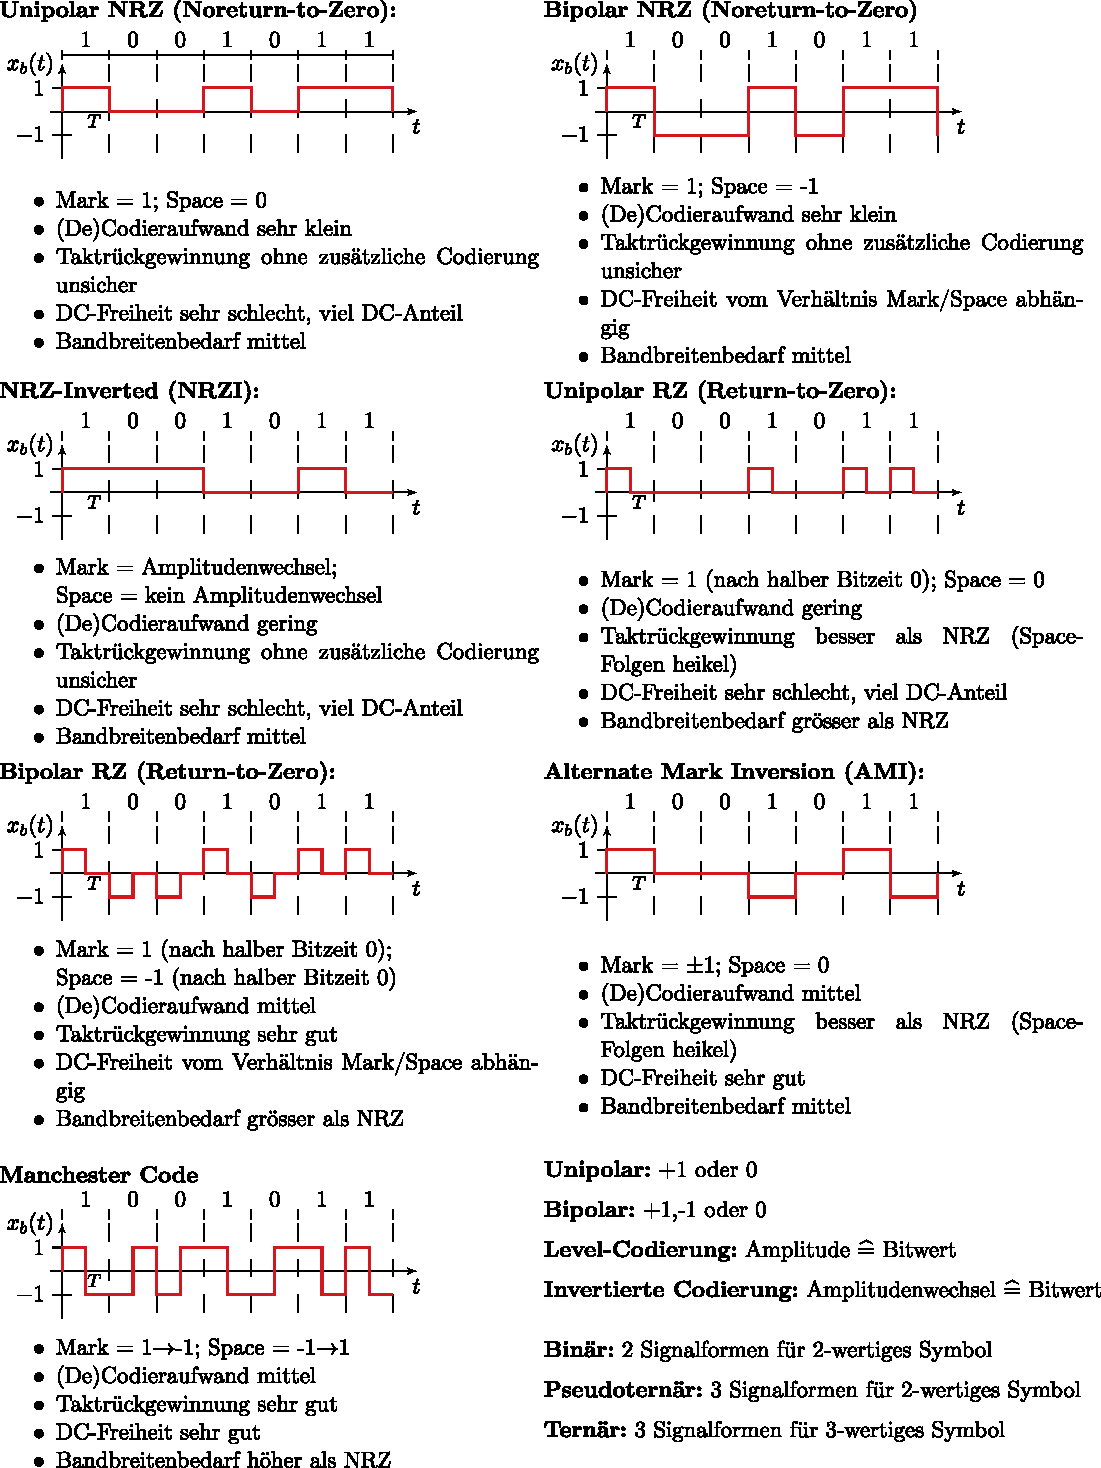
\includegraphics{content/08_digsigtransmit/leitungscodierung.pdf}\\
	\newpage
\begin{tabularx}{\linewidth}{p{.1\linewidth} p{.4\linewidth} p{.1\linewidth} p{.4\linewidth}}
	NRZ: & ZOH über ganze Symbolzeit & Mark: & übertragenes Bit mit Wert 1 \\
	RZ: & ZOH nur über halbe  Symbolzeit & Space: & übertragenes Bit mit Wert 0 \\
	 & Scrambler S. 96, Bitstopfen (bit stuffing) S.  &96 & 8b10b Codierung S. 97
\end{tabularx}

\subsection{Bandbreitenbedarf von PCM (Pulse-Code-Modulation) S. 104}

Bandbreitenbedarf ist nicht explizit berechenbar, er ist abhängig von Anzahl Bits pro Symbolzeit und\\ Leitungscodierungsart.

\subsubsection{min. Bandbreitenbedarf im Binären Fall S.105}
\begin{tabularx}{.6\linewidth}{m{.4\linewidth} m{.3\linewidth} m{.3\linewidth}}
	Samplingrate: 			& $f_s > 2\cdot B_m$ 	&
	\multirow{4}{.75\linewidth}{\begin{minipage}{\linewidth}
		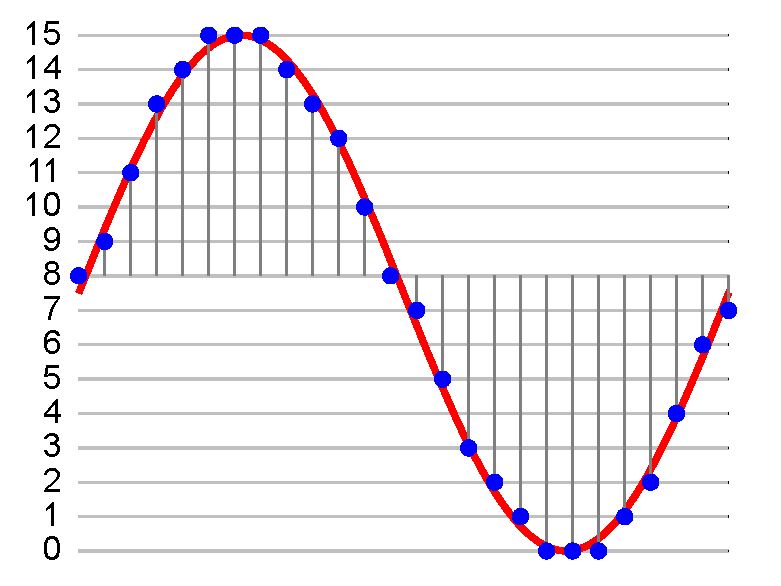
\includegraphics[width=\linewidth]{content/08_digsigtransmit/pcm.pdf}\\
		4 Bit PCM 
	\end{minipage}} \\
	Bitrate: 				& $n\cdot f_s > 2n \cdot B_m$ \\
	minimale Bandbreite:	& \efbox[linecolor=red]{$B_{PCM} = \frac{1}{2} \cdot n \cdot f_s > n\cdot B_m$} \\
	effektiver Bandbreitebedarf: (weil es keine idealen Filter gibt) & \efbox[linecolor=red]{$B_{eff} > B_{PCM} > n \cdot B_{m}$}
\end{tabularx}

\subsection{Pulsformfilter S. 106}
\subsubsection{Intersymbol Interferenz (ISI)}
	\begin{list}{$\bullet$}{\setlength{\itemsep}{0cm} \setlength{\parsep}{0cm} \setlength{\topsep}{0cm}} 
	\item Wenn digitale Signale mit Rechteckimpulsen dargestellt werden, müssen die Pulse verbreitert werden um Bandbreite zu sparen.
	\item Interferenz + weitere Störungen = Bitfehler beim Empfänger
	\item Verarbeitung führt zu Überlappung benachbarter Pulse $\rightarrow$ Intersymbol Interferenz
	\item Bereich für korrekte Entscheidungsschwelle wird verkleinert (vertikale Augenöffnung)
\end{list}
\textbf{Massnahmen gegen Intersymbol Interferenz}: Abtastzeitpunkt muss vom Empfänger optimal gewählt werden (horizontale Augenöffnung). Sendepulse so wählen, dass sich das Auge maximal öffnet (zum Abtastzeitpkt soll keine Interferenz von Nachbarsymbolen vorhanden sein). Synchronisation Sender und Empfänger.
\subsubsection{Erstes Nyquist-Kriterium S. 106}
Wenn erstes Nyquist-Kriterium erfüllt ist, kann Intersymbol-Interferenz eliminiert werden.\\
\begin{tabularx}{\linewidth}{X X}
	\begin{minipage}{\linewidth}
		\textbf{Im Zeitbereich}\\
		\boxedeq{\begin{split} \sum_{n=-\infty}^{\infty} s_p(n\cdot T) \cdot \delta(t-n\cdot T) = s_{p0} \cdot \delta(t) \end{split}} \\
		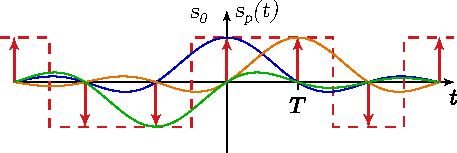
\includegraphics{content/08_digsigtransmit/1nyquisttimedomain.pdf}\\
		Signal muss mit $f_s = \frac{1}{T_s} = \frac{1}{T}$ abgetastet werden. 
	\end{minipage}
	&
	\begin{minipage}{\linewidth}
		\textbf{Im Frequenzbereich}\\
		\boxedeq{\begin{split} \frac{1}{T} \sum_{n=-\infty}^{\infty} S_p(\omega - n\cdot \frac{2\pi}{T}) \cdot \delta(t-n\cdot T) = s_{p0} \end{split}}\\
		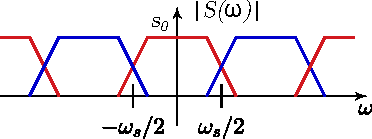
\includegraphics{content/08_digsigtransmit/1nyquistfrequencydomain.pdf}\\
		Das Spektrum muss summiert konstant sein!\\
		Minimale Bandbreite: $B_{min} = \frac{1}{T} = \frac{f_s}{2}$
	\end{minipage}
\end{tabularx}
\subsubsection{Zweites Nyquist-Kriterium S. 111}
Das Augendiagramm soll nicht nur bezüglich der Amplitude, sondern auch bezüglich deR Zeitachse maximal geöffnet sein.\\
Zusätzlich zu den Nullstellen bei $nT$ muss die Impulsform $s_p(t)$ auch Nullstellen haben bei:\\
$\pm \frac{3}{2}T; \pm \frac{5}{2}T; \pm \frac{7}{2}T; ...$\\
Von der Gruppe der Raised-Cosine Pulsen erfüllen nur diejenigen mit Roll-off Faktor $\alpha = 1$ das zweite Nyquist-Kriterium.

\subsubsection{Raised Cosine Pulse S. 107}
\begin{tabularx}{\linewidth}{m{.5\linewidth} m{.5\linewidth}}
	\boxedeq{\begin{split} s_{rc} = \frac{\sin\frac{\pi}{T}t}{\frac{\pi}{T}t} \cdot \frac{\cos\alpha \frac{\pi}{T}t}{1-(2\alpha \frac{\pi}{T}t /\pi)^2} \end{split}}
	&
	Roll-off Faktor $\alpha$ : $0 \geq \alpha \geq 1$
\end{tabularx}

\begin{tabularx}{\linewidth}{m{.65\linewidth} m{.35\linewidth}}
	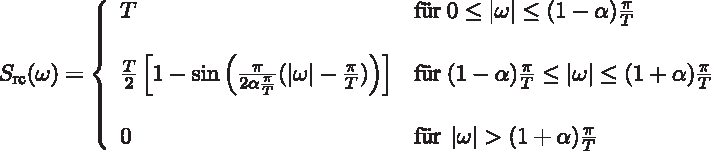
\includegraphics{content/08_digsigtransmit/fancyRCequation.pdf}
	&
	\textbf{Bandbreite:} $B=\frac{f_s}{2} \cdot (1+\alpha) $
\end{tabularx}

\begin{tabularx}{\linewidth}{m{.31\linewidth} m{.36\linewidth} m{.24\linewidth}}
	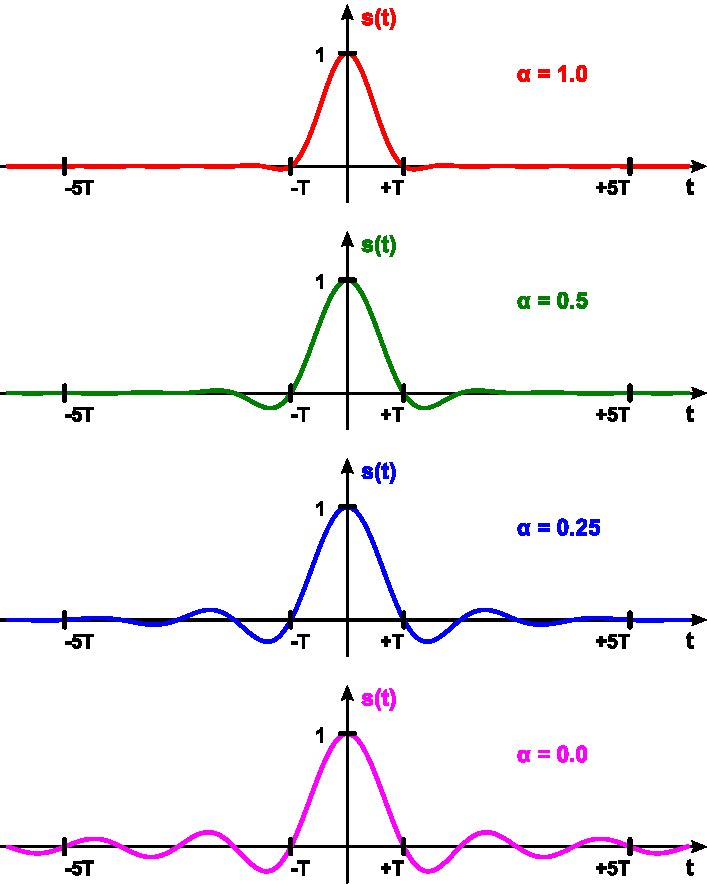
\includegraphics[width=\linewidth]{content/08_digsigtransmit/abbildung7_11.pdf}
	&
	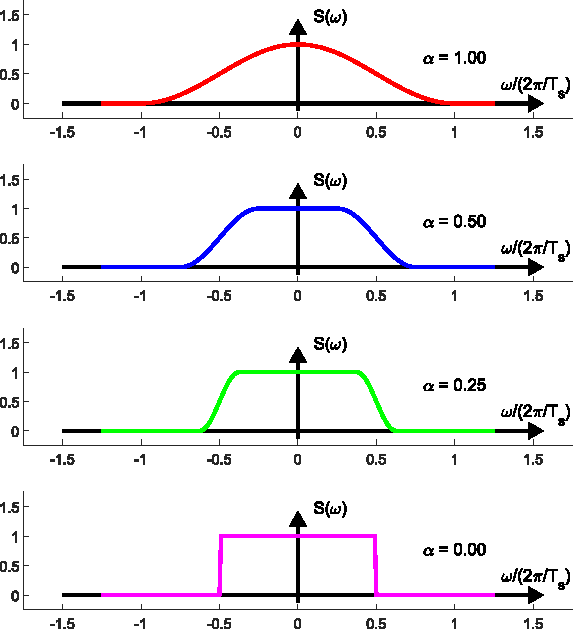
\includegraphics[width=\linewidth]{content/08_digsigtransmit/abbildung7_12.pdf}
	&
	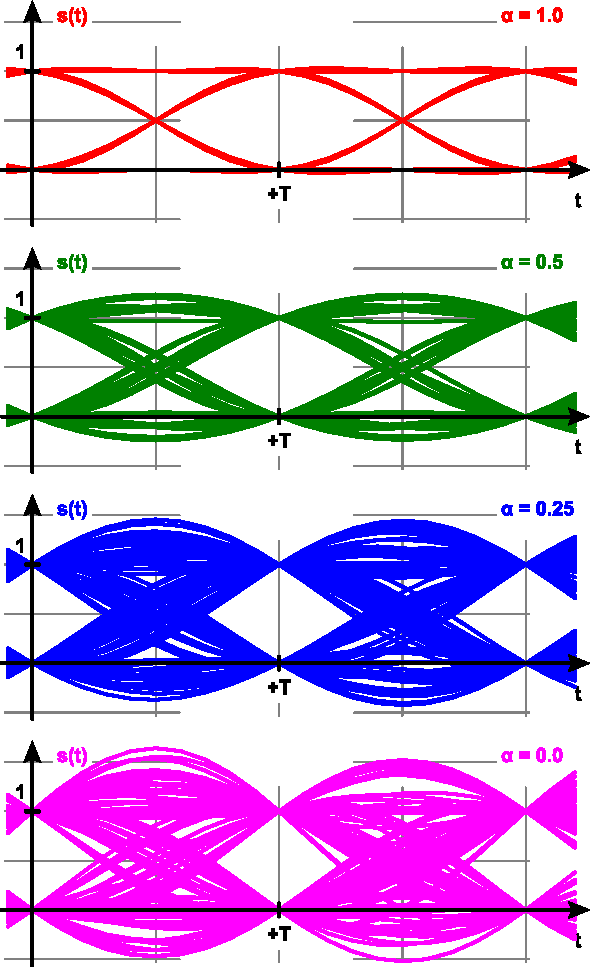
\includegraphics[width=\linewidth]{content/08_digsigtransmit/abbildung7_13.pdf}
\end{tabularx}

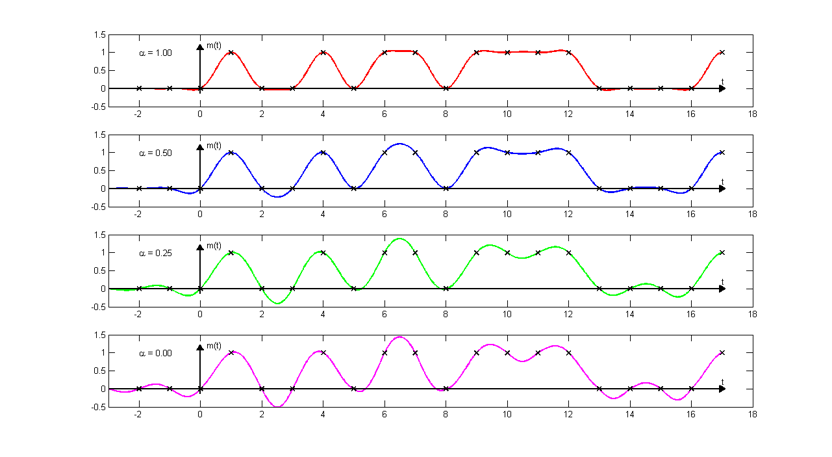
\includegraphics[trim=2cm 1cm 2cm 0cm,clip]{content/08_digsigtransmit/RC_mt_timedomain.png}

\subsection{Digitale Modulation von Trägersignal S. 111}
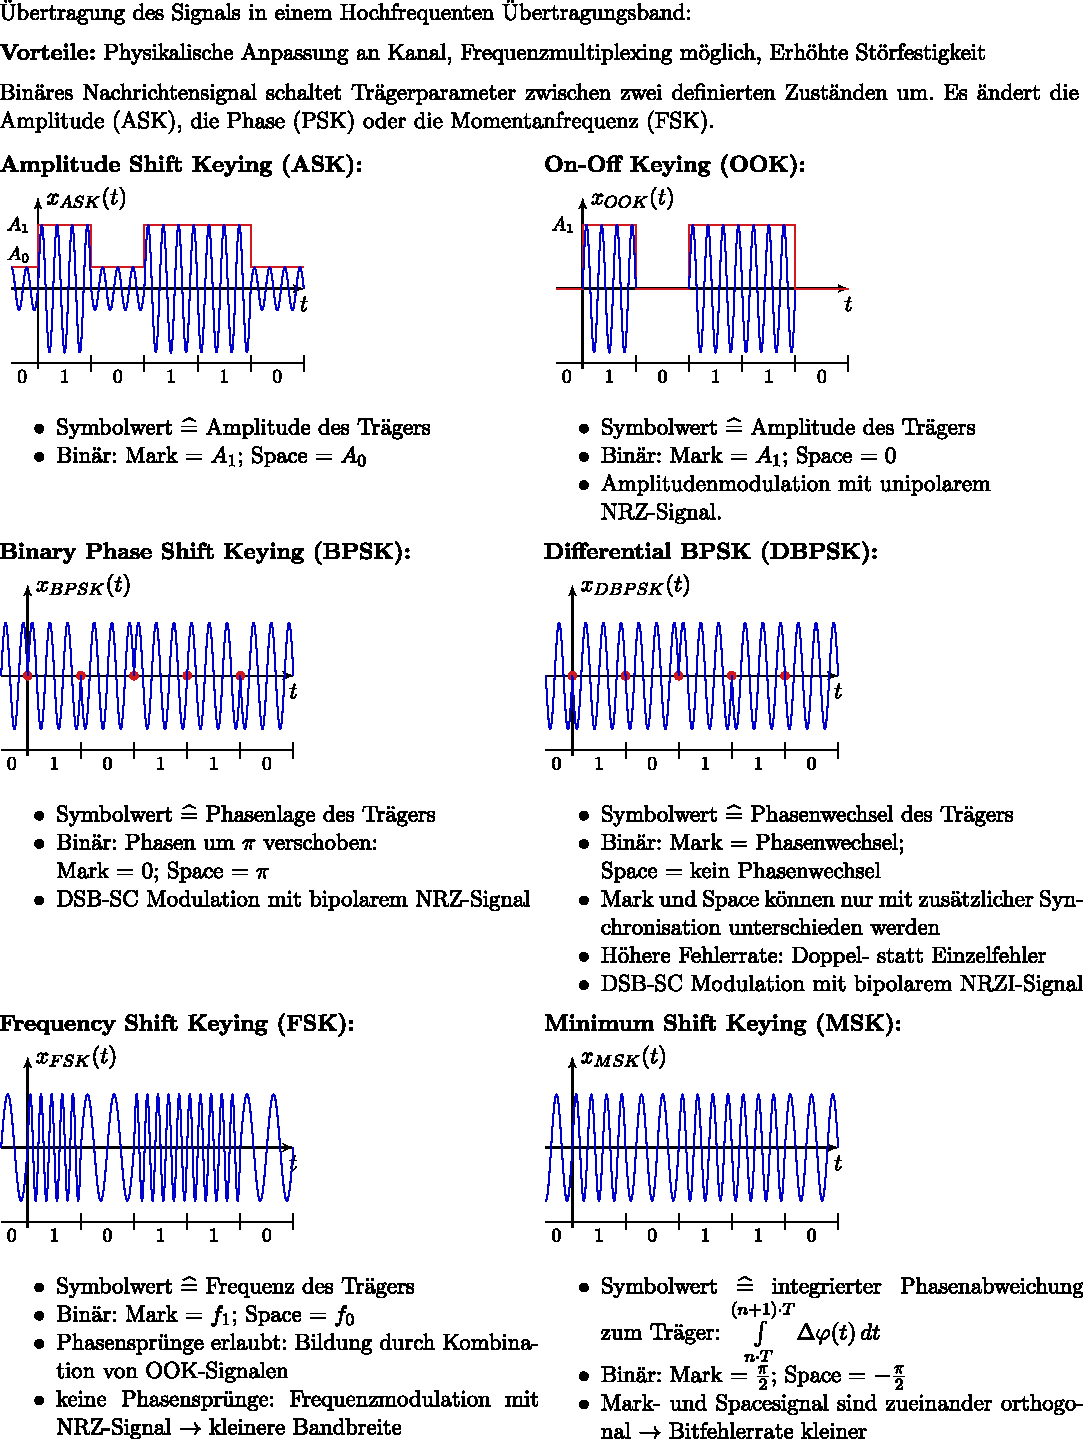
\includegraphics{content/08_digsigtransmit/digModCarrier.pdf}

\subsection{Äquivalente Basisbanddarstellung von Bandpassignalen S. 116}
Ein Bandpasssignal kann als Basisbandsignal aufgefasst werden, welches zur (positiven) Trägerfrequenz $+f_c$ hin verschoben wird.\\
\boxedeq{\begin{split} x_{BP} = \Real(x_{eq}(t) \cdot e^{j\omega_ct}) = a(t)\cos(\omega_ct)-b(t)\sin(\omega_ct) \;\;\; | \;\;\; x_{eq} = a(t) +jb(t)\end{split}}

$X_{BP}(\omega)$ symmetrisch zu $\omega_c \;\;\; \rightarrow \;\;\; x_{eq}(t)$ reell\\
$X_{BP}(\omega)$ asymmetrisch zu $\omega_c \;\;\; \rightarrow \;\;\; x_{eq}(t)$ komplex

\subsubsection{Basisbanddarstellung}
Ist das Nachrichtensignal ein Rechteck, beschränkt sich die Basisbanddarstellung auf einzelne Werte in der komplexen Ebene.\\
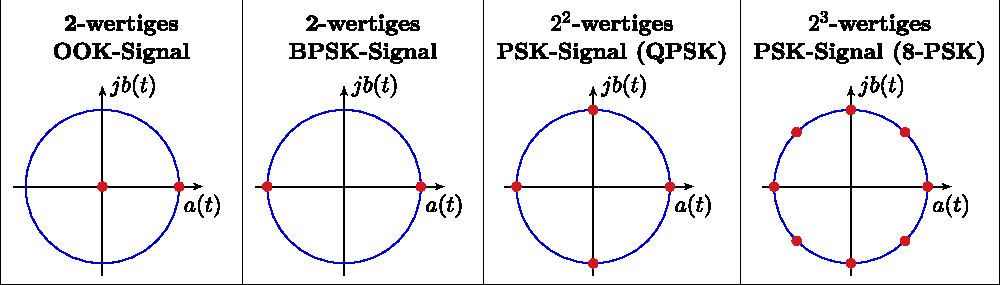
\includegraphics{content/08_digsigtransmit/basisbanddarstellungen.pdf}

\subsection{Quadratur Amplitudenmodulation (QAM) S. 118}
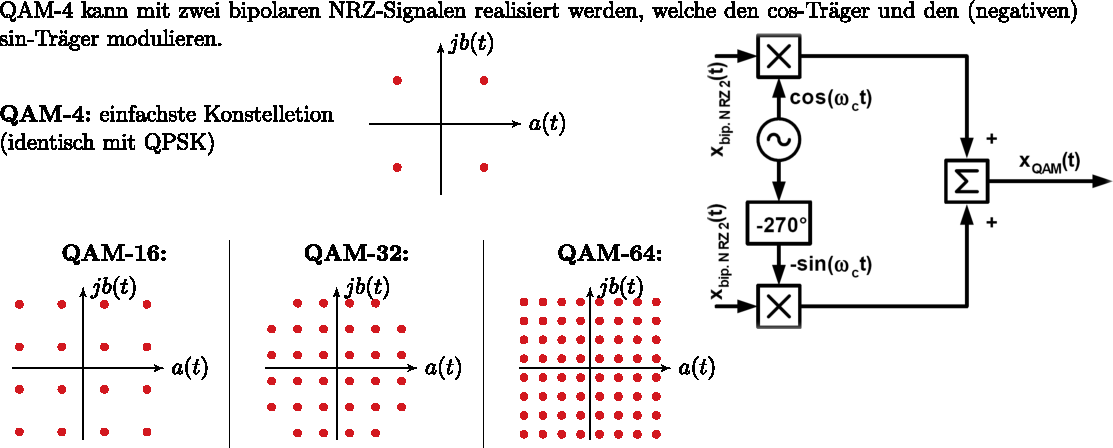
\includegraphics{content/08_digsigtransmit/qam.pdf}

Anzahl Bit pro Symbol $= floor(\log_2(\text{Anzahl Punkte}))$ \hspace{.5cm} \efbox[linecolor=red]{$B_{QAM-rc} = f_s(1+\alpha) \;\;\; |\;\; \alpha \text{ Roll-off Faktor}$}

\subsubsection{Gray-Codierung von QAM}
\begin{minipage}{.4\linewidth}
	Bitfehler entstehen, wenn bei beeinträchtigtem
	Empfang falsche Amplitudenwerte decodiert wer-
	den. Dabei ist es am Wahrscheinlichsten, dass ein
	benachbartes Feld detektiert wird.
	Durch den \textbf{Gray-Code} können \textbf{mehrfache Bit-
	fehler vermieden} werden (zwischen Nachbarn
	ändert nur 1 Bit).
\end{minipage}
\hspace{1cm}
\begin{minipage}{.6\linewidth}
	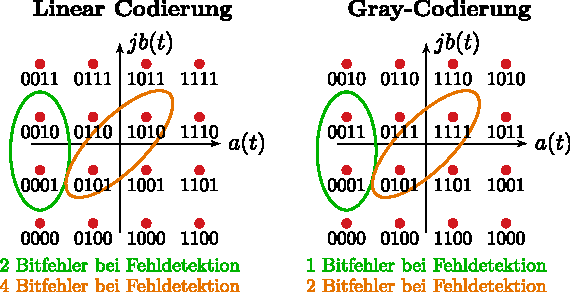
\includegraphics[width=.8\linewidth]{content/08_digsigtransmit/graycodeqam.pdf}
\end{minipage}

\subsubsection{Pulsformfilter zur QAM S. 121}
Rechteckige Signale im Basisband $\rightarrow$ hoher Bandbreitenbdarf im Basisband $\rightarrow$ doppelter Bandbreitenbedarf im Basisband!\\
Bandbreite im Basisband kann mit Pulsformfilter gezielt reduziert werden.\\
Geeigenter Filter: \textbf{Raised-Cosine Filter}

\paragraph{Gefilterte Übergänge}
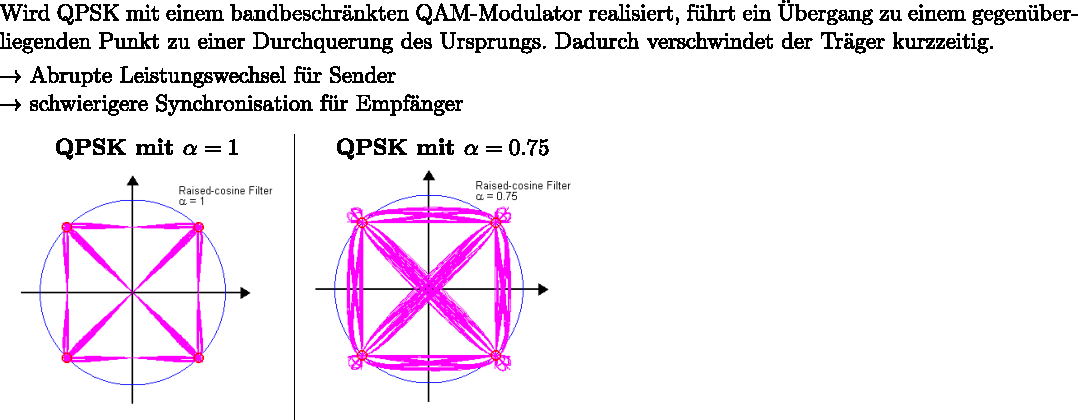
\includegraphics{content/08_digsigtransmit/gefilterteuebergaenge.pdf}

\paragraph{Filterung mit Offset}
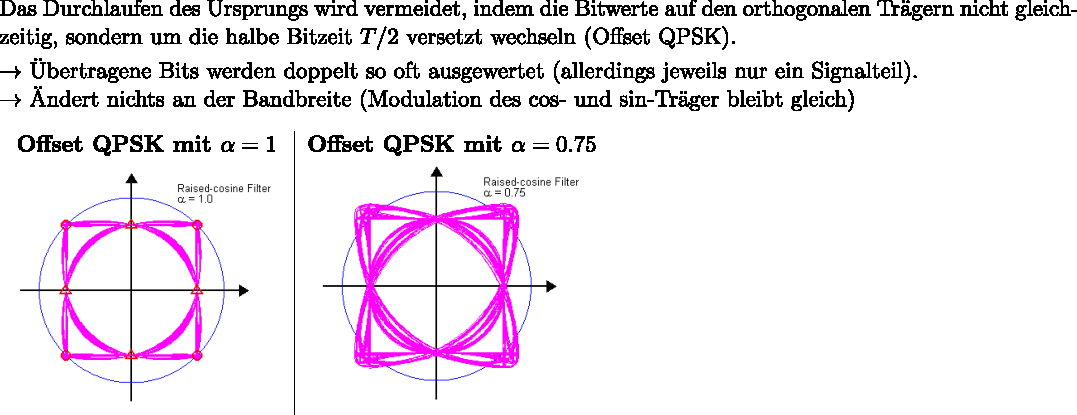
\includegraphics{content/08_digsigtransmit/filterungmitoffset.pdf}
